
\documentclass[fleqn,12pt]{SelfArx} % Document font size and equations flushed left

\usepackage[english]{babel} % Specify a different language here - english by default

\usepackage{lipsum} % Required to insert dummy text. To be removed otherwise

%----------------------------------------------------------------------------------------
%	COLUMNS
%----------------------------------------------------------------------------------------

\setlength{\columnsep}{0.55cm} % Distance between the two columns of text
\setlength{\fboxrule}{0.75pt} % Width of the border around the abstract

%----------------------------------------------------------------------------------------
%	COLORS
%----------------------------------------------------------------------------------------

\definecolor{color1}{RGB}{94,192,150} % Color of the article title and sections
\definecolor{color2}{RGB}{236,124,63} % Color of the boxes behind the abstract and headings

%----------------------------------------------------------------------------------------
%	HYPERLINKS
%----------------------------------------------------------------------------------------

\usepackage{hyperref} % Required for hyperlinks
\hypersetup{hidelinks,colorlinks,breaklinks=true,urlcolor=color2,citecolor=color1,linkcolor=color1,bookmarksopen=false,pdftitle={Title},pdfauthor={Author}}

%----------------------------------------------------------------------------------------
%	ARTICLE INFORMATION
%----------------------------------------------------------------------------------------

\JournalInfo{Deep Micro Systems, 2018} % Journal information
\Archive{Smart Cities} % Additional notes (e.g. copyright, DOI, review/research article)

\PaperTitle{DeMS White Paper} % Article title

\Authors{Stanley Salvatierra\textsuperscript{1}*, Alvaro Hurtado\textsuperscript{2}} % Authors
\affiliation{\textsuperscript{1}\textit{Chief Technology Officer, DeMS, Smart Cities}} % Author affiliation
\affiliation{\textsuperscript{2}\textit{Chief Executive Officer, DeMS, Smart Cities}} % Author affiliation
\affiliation{*\textbf{Stanley Salvatierra}: s.salvatierra@deepmicrosystems.com} % Corresponding author

\Keywords{Computer Vision --- Smart Cities --- Offline computing --- Artificial Intelligence} % Keywords - if you don't want any simply remove all the text between the curly brackets
\newcommand{\keywordname}{Keywords} % Defines the keywords heading name

%----------------------------------------------------------------------------------------
%	ABSTRACT
%----------------------------------------------------------------------------------------

\Abstract{\lipsum[1]~}

%----------------------------------------------------------------------------------------

\begin{document}

\flushbottom % Makes all text pages the same height

\maketitle % Print the title and abstract box

\tableofcontents % Print the contents section

\thispagestyle{empty} % Removes page numbering from the first page

%----------------------------------------------------------------------------------------
%	ARTICLE CONTENTS
%----------------------------------------------------------------------------------------

\section*{Introduction} % The \section*{} command stops section numbering

\addcontentsline{toc}{section}{Introduction} % Adds this section to the table of contents

Privacy concerns, low internet conectivity and low computational power are some of the main reasons to improve real time video analisys to work in local devices.
%------------------------------------------------

\section{Who We Are}

Deep Micro Systems is a Bolivian Start up in the field of computer vision and Smart cities. Our mission is to  expand the awareness and knowledge industry and governments to smart cities, providing security, efficiency and generating solutions to critical problems in a measurable and sustainable way.

\paragraph{Road Insecurity} The high numbers in roads accidents is currenlty a great concern for Bolivian government. New technologies are needed in order to reduce this huge numbers. As Internet connectivity in Bolivia is expensive and low efficient compared to our neighbor countries, the need of offline processing is a major concern. In order to achieve this Deep Micro Systems designed an All In One Device capable of detecting traffic Infringements and generate valuable data for city planning.

With the main purpose of generating security in roads and streets, Our camera is capable of detecting events in real time video.

\paragraph{Applications of computer vision} Besides road infringement detection, Deep Micro Systems works with computer vision, and it's variety of applications in industry and government. Some of other projects for Deep Micro Systems in the short term are:

\begin{itemize}[noitemsep] % [noitemsep] removes whitespace between the items for a compact look
\item Optimal city design, parking, roads and flows
\item Traffic accidents forecast
\item Smart traffic light managing
\end{itemize}

\subsection{Low cost, effective devices}

The lowering costs of pocket computers and the increasing power and efficiency of machine learning techniques allow to build small devices capable of solve huge problems in cities and in the industry

\begin{figure}[ht]\centering
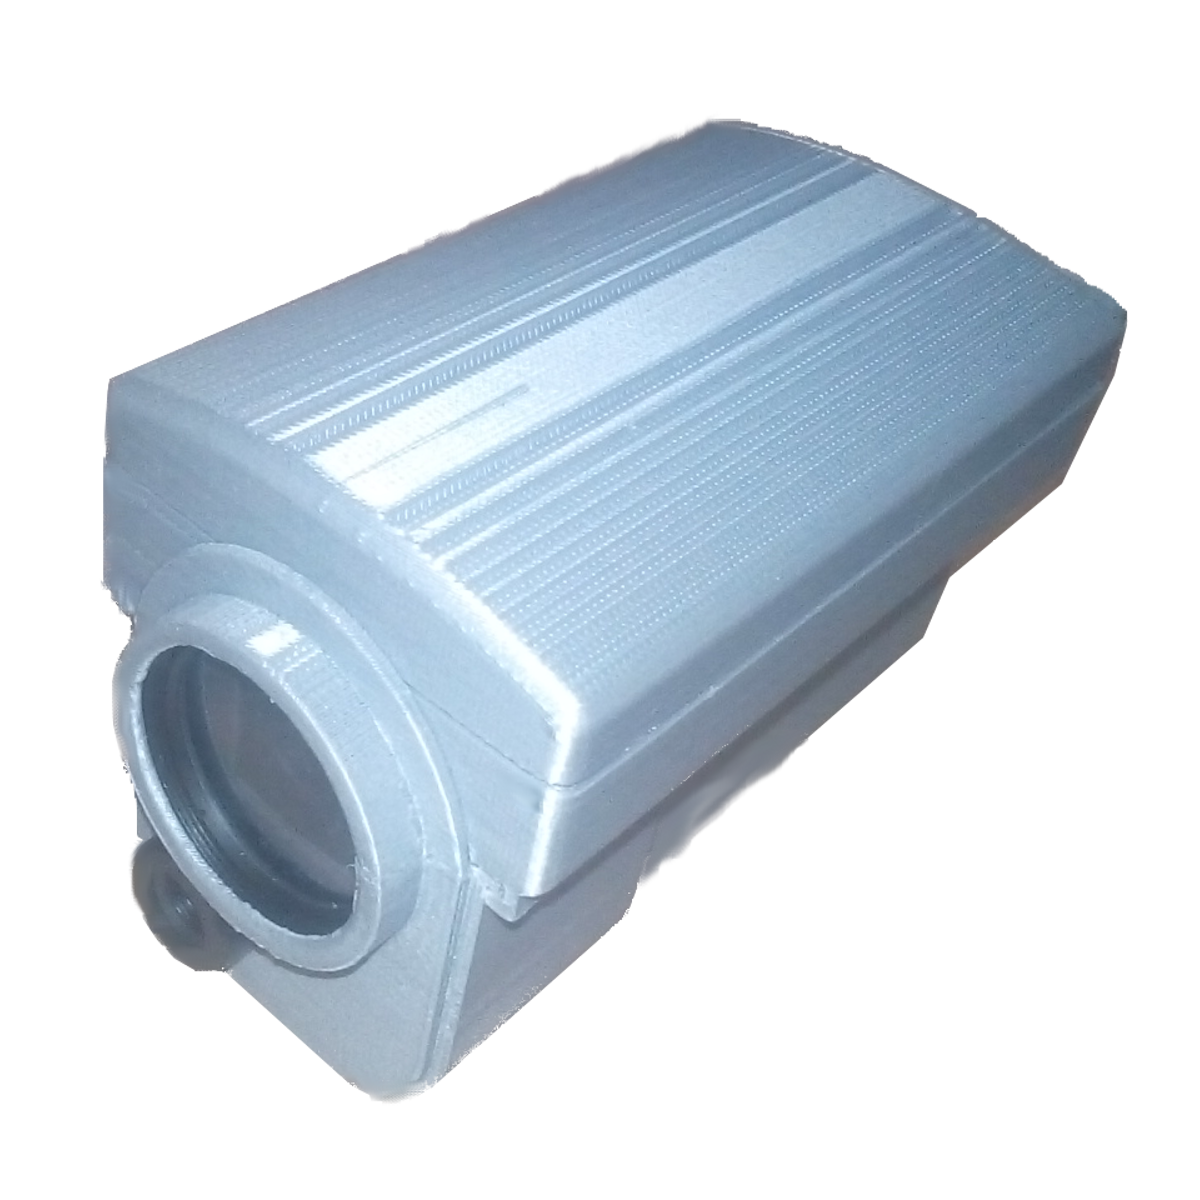
\includegraphics[width=\linewidth]{lucam_005}
\caption{All-In-One computer vision device}
\label{fig:results}
\end{figure}

Currently Lu-Cam, our smart traffic enforcement camera is a 8x9x16 cm device capable, as seen in figure \ref{fig:results}, and it is capable of detecting events in real time video.

%------------------------------------------------

\section{On the Edge Computing}

\lipsum[10] % Dummy text

\subsection{Subsection}

\lipsum[11] % Dummy text

\begin{table}[hbt]
\caption{Table of Grades}
\centering
\begin{tabular}{llr}
\toprule
\multicolumn{2}{c}{Name} \\
\cmidrule(r){1-2}
First name & Last Name & Grade \\
\midrule
John & Doe & $7.5$ \\
Richard & Miles & $2$ \\
\bottomrule
\end{tabular}
\label{tab:label}
\end{table}

\subsubsection{Subsubsection}

\lipsum[12] % Dummy text

\begin{description}
\item[Word] Definition
\item[Concept] Explanation
\item[Idea] Text
\end{description}

\subsubsection{Subsubsection}

\lipsum[13] % Dummy text

\begin{itemize}[noitemsep] % [noitemsep] removes whitespace between the items for a compact look
\item First item in a list
\item Second item in a list
\item Third item in a list
\end{itemize}

\subsubsection{Subsubsection}

\lipsum[14] % Dummy text

\subsection{Further applications}

\lipsum[15-23] % Dummy text

%------------------------------------------------
\phantomsection
\section*{Acknowledgments} % The \section*{} command stops section numbering

\addcontentsline{toc}{section}{Acknowledgments} % Adds this section to the table of contents

So long and thanks for all the fish \cite{Cavigelli:2017:CCI:3131885.3131906}.

%----------------------------------------------------------------------------------------
%	REFERENCE LIST
%----------------------------------------------------------------------------------------
\phantomsection
\bibliographystyle{unsrt}
\bibliography{sample}

%----------------------------------------------------------------------------------------

\end{document}